\documentclass{article}

\usepackage{amsmath, amsfonts, amssymb}
\usepackage{graphicx}
\usepackage{fancyvrb}

\title{Homework 9}
\author{Matthew Dupraz}

\begin{document}

\maketitle

\subsection*{(a)}

Let $x_i = ih$ for $i \in \{0, \dots, N\}$ and $h = 1/N$.
We will apply the composite trapezoidal rule to approximate
the solution at each $x_i$:
\begin{align*}
	\int_0^1 k(x_i, y)u(y) dy &\approx
	Q^{(1)}_h[k(x_i, \cdot)u(\cdot)]\\
	&= \sum_{j=0}^{N-1}\frac{x_{j+1} - x_j}{2}[
	k(x_i, x_j)u(x_j) + k(x_i, x_{j+1}u(x_{j+1}))]\\
	&= \frac{h}{2}\sum_{j=0}^{N-1}[
	k(x_i, x_j)u(x_j) + k(x_i, x_{j+1}u(x_{j+1}))]\\
	&= \frac{h}{2}k(x_i, 0)u(0) + \frac{h}{2}k(x_i,1)u(1)
	+ h\sum_{j=1}^{N-1}k(x_i, x_j)u(x_j)
\end{align*}

Consider $\vec{f} = [f(x_0, \dots, f(x_N)]^T$, we'll find values
$\vec(u) = [u(x_0), \dots, u(x_N)]^T$ such that
\begin{equation*}
	Q_h^{(1)}[k(x_i, \cdot)u(\cdot)] = f(x_i) ~~
	\forall i \in \{0, \dots, N\}
\end{equation*}
If we let
\begin{equation*}
	A = \begin{bmatrix}
		\frac{h}{2}k(x_1, 0) & hk(x_1, x_1) & \cdots &
		hk(x_1, x_{N-1}) & \frac{h}{2} k(x_1, x_N)\\
		\vdots & \vdots & & \vdots & \vdots\\
		\frac{h}{2}k(x_N, 0) & hk(x_N, x_1) & \cdots &
		hk(x_N, x_{N-1}) & \frac{h}{2} k(x_N, x_N)\\
	\end{bmatrix},
\end{equation*}
then using the formula for the composite trapezoidal rule we found
above, this is equivalent to $A\vec{u} = \vec{f}$

\subsection*{(b)}
We can see that if we let
\begin{equation*}
	D =
	\begin{bmatrix}
		\frac{h}{2} & & & & \\
		 & h & & & \\
		 & & \ddots & & \\
		 & & & h & \\
		 & & & & \frac{h}{2}
	\end{bmatrix},
\end{equation*}
then $A = KD$. And so
\begin{equation*}
	A\vec{u} = \vec{f} \iff KD\vec{u} = \vec{f}
		\iff D\vec{u} = K^{-1}\vec{f}.
\end{equation*}
By definition of $f_z$ and the formula for the composite trapezoidal
rule we found in part (a), we have that
\begin{equation*}
	f_z = [k(z, x_0)~\cdots~k(z, x_N)]D\vec{u}
\end{equation*}
and so we conclude
\begin{equation*}
	f_z = [k(z, x_0)~\cdots~k(z, x_N)]K^{-1}\vec{f}
\end{equation*}

\subsection*{(c)}
Let $i \in \{0, \dots, N\}$. If $K$ is invertible, then
\begin{equation*}
	[k(x_i, x_0)~\cdots~k(x_i, x_N)]K^{-1} = \vec{e_i}
\end{equation*}
since $[k(x_i, x_0)~\cdots~k(x_i, x_N)]$ is the $i$-th column of
the matrix $K$.
Hence
\begin{equation*}
	f_{x_i} = [k(x_i, x_0)~\cdots~k(x_i, x_N)]K^{-1}\vec{f}
	= \vec{e_i}\cdot\vec{f} = f_i = f(x_i)
\end{equation*}

\subsection*{(d)}

\begin{Verbatim}[frame=single,
	label=\textsc{Matlab} code - approximate.m]
function [y]=approximate(f, N, z, lambda)
    k = @(x, y) exp(-(x-y).^2/2);
    x = (0:N)/N;
    K = k(x', x);
    % regularize matrix K
    K = K + lambda*eye(size(K));
    Z = k(z', x);
    y = Z*(K\f(x'));
\end{Verbatim}

\subsection*{(e)}

Applying the above function to $f_1(x) = \exp(x)$ and
$f_2(x) = \sqrt{|1/2 - x|}$ produced the following
plots:

\begin{center}
	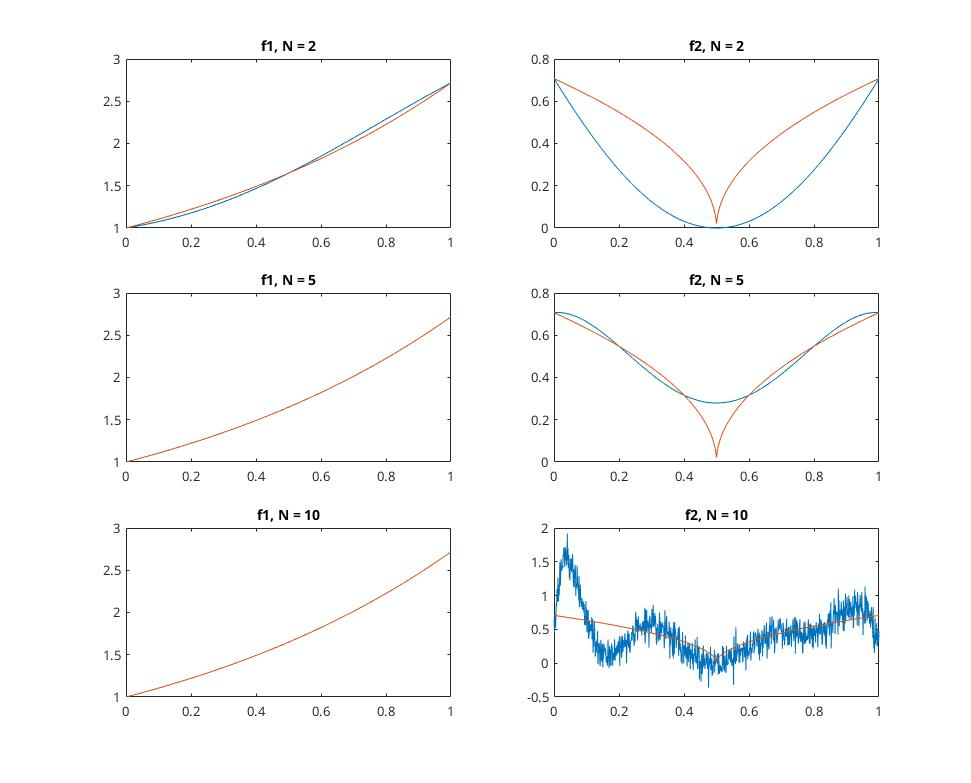
\includegraphics[width=\textwidth]{figure.jpg}
\end{center}

The errors obtained are then
\begin{center}
\begin{tabular}{ | c | c c c |}
\hline
 & $N = 2$ & $N=5$ & $N=10$ \\
 \hline
$f_1$ & 0.0624 & 0.0002 & 0.0000002 \\
$f_2$ & 0.3228 & 0.2570 & 1.2402\\
\hline
\end{tabular}
\end{center}
Below follows the script used to obtain these plots and
error values:

\begin{Verbatim}[frame=single,
	label=\textsc{Matlab} code - main.m]
% We define the functions we use
f1 = @(x) exp(x);
f2 = @(x) sqrt(abs(1/2 - x));

% Functions and values of N we want to
% iterate over
fs = {f1, f2};
Ns = [2, 5, 10];

% Evaluation points
z = linspace(0, 1, 1000);

errors = zeros(2, 3);

for i=1:2
    f = fs{i};
    y = f(z);
    for j=1:3
        N = Ns(j);
        % Calculate approximated values
        approx_y = approximate(f, N, z, 0)';
        errors(i, j) = max(abs(approx_y - y));

        % Display results
        subplot(3, 2, i + 2*(j-1));
        plot(z, approx_y);
        hold on;
        plot(z, y);
        title(sprintf("f%g, N = %g", i, N));
    end
end

disp(errors);

% We use lambda = 10^(-14)
corrected_y = approximate(f2, 10, z, 10^(-14))';
error = max(abs(f2(z) - corrected_y));
disp(error);
\end{Verbatim}

\subsection*{(f)}

For $N=10$, the matrix $K$ has a condition number equal to
$\kappa_\infty = 3.3445\mathrm{e}{+17}$, which is way too high to expect any
accuracy in calculating $K^{-1}\vec{f}$ (indeed the upper bound
obtained in theorem 4.23 becomes useless when
$\kappa > 10^{16}$ as then the upper bound on the relative error
is larger than $1$). We try to decrease the
condition number of $K$ by adding $\lambda I_n$ to it for a small
value of $\lambda$. Experimentally I found that setting
$\lambda = 10^{-14}$ gives us an error of about
$0.098 < 10^{-1}$ for $N=10$. 

\end{document}
